\chapter{\hspace*{3pt} Related Concepts}
\label{chapter:related-concepts}



This chapter introduces the theoretical concepts used to contextualize the research described in this thesis.

The concepts related to Collective Intelligence and Collective construction of Knowledge are essential for understanding the motivation to choose an approach that uses the knowledge of the contributors of Wikipedia, rather than experts. The description of Wikipedia and its features is central to the understanding of the organization of this body of knowledge, as well as the possibilities and challenges that emerge from decoding  the underlying structure. 
The concepts related to Information Retrieval and Extraction are essential to understanding the tasks applied in the proposed solution to extract the entities and the categories from the text-resources.
We also provide some general information about natural language processing (NLP) techniques that are applicable to our categorization method. 
This chapter ends with an overview of the concept and methods for the automatic classification of textual resources, as it is the primary goal of the research presented in this thesis. 

\section{\hspace*{3pt}Natural Language}

Natural language is any language developed naturally by the human being, in an unpremeditated way, as a result of the natural ease of language processing by the human intellect \cite{chomsky1975logical}. Spoken, written and sign languages are examples of natural languages. 
All the elements of a language are linked together by a variety of relations, and for that reason, they can be considered systems. Although the assimilation language occurs naturally by humans, it is a system of remarkable complexity \cite{chomsky1975logical}. 
As it is the expression of the culture of a society, developed through the generations and in different situations, it does not constitute a system of rigid rules that can be trivially implemented and interpreted by computers.


Unlike humans, machines are designed to perform well-defined tasks from specific instructions. A computer is not by itself an intelligent machine in the sense that it can not learn from its own experience to improve its future behavior. On the contrary, a computer is only capable of strictly performing tasks that are delegated to it and that are part of the set of actions that it can perform. In this sense, it is necessary to understand what kind of instructions can be executed by the computers so that we can program them - instruct them with the sequence of actions necessary to solve a particular problem so that they carry out the task in the desired way.
\subsection{\hspace*{3pt}Natural Language Processing - NLP}

 

\gls{nlp} consists of the development of mathematical and computational models of various aspects of language, to make possible the development of a wide range of systems that rely on information expressed in natural language \cite{joshi1991natural}.


\gls{nlp} has the general objective of processing human language so that it is understandable by the computer. Among the essential areas of \gls{nlp} we can highlight: the recognition of voice, the recognition of writing and the reproduction of voice from the text. \gls{nlp} encompasses several and complex areas of knowledge, hence the  researches in this field are interdisciplinary, involving concepts of computer science, linguistics, logic, and psychology.


\subsection{\hspace*{3pt}Text-based Resources}
Structured resources are machine-readable resources that encode relationships of various types according to the level of information \cite{hovy2013collaboratively}. Structured resources are of high quality as they are built from the knowledge of domain experts, lexicographers, and linguists. However, structured resources are limited because they require significant efforts in creation and updating. Because they are built manually, they depend on the availability of experts to extend their coverage and to keep them up to date on recent events. Moreover, knowledge encoded in one language is not transferable to others, requiring a new effort for each new language.

The most common structured resources are:

\begin{itemize}


\item Thesaurus: collections of related terms;
\item Taxonomies: Hierarchical structures of classification of terms;
\item Ontologies: knowledge models that include concepts, relations of different types, rules and axioms.
\end{itemize}

Unstructured resources are collections of texts that have no formalized knowledge and are machine readable only as sequences of characters and words. Different statistical models can extract knowledge from unstructured collections, and the massive amount of texts available on the \gls{www} enables the construction of knowledge bases of excellent coverage. However, they are limited by the lack of texts that demonstrate common-sense knowledge \cite{hovy2013collaboratively}. Also, statistical models are not able to issue knowledge with quality equivalent to the resources built by specialists.

The authors conclude that the limitations of unstructured resources are complementary to the limitations of structured resources. While unstructured resources enable broad coverage with low quality, structured resources have high quality but low coverage. Semistructured resources constructed collaboratively on the \gls{www} encode the knowledge voluntarily made available by users of these resources, covering different areas of knowledge and having quality comparable to that obtained from specialists. The semi-structured resources mentioned by the authors are Wiktionary, Flickr, Twitter, Yahoo! Answers and, with greater emphasis on the Wikipedia \cite{hovy2013collaboratively}.




\section{\hspace{3pt}Information Retrieval}

\gls{ir} systems are mostly known for their searching ability, where a user states an information need and the system provides the user with a response to this information need in return. IR is a large academic field and encompasses several topics like browsing or filtering documents, processing of retrieved documents and clustering or classifying documents according to their content \cite{Manning:2008}, Manning defines \gls{ir} as:

\begin{displayquote}
\say{finding material (usually documents) of an unstructured nature (usually text) that satisfies an information need from within large collections (usually stored on computers)}\cite{Manning:2008}. 
\end{displayquote}

A system can increase its precision when retrieving the users' information need if it indexes well-representing features of the text. As the collection of documents expand, automatic techniques that can extract these features become crucial.  Text Classification techniques can provide an output that can be representative of a research document, allowing for IR systems to handle the indexing and retrieval process.

\section{\hspace*{3pt}Information Extraction}

\gls{ie} is the process of automatically extracting particular information entities or the relationship between different information entities from a source \cite{sarawagi2008information} and presenting it in a structured form. The source of information can be structured like a relational database, semi-structured like an HTML document or unstructured as free text from an academic paper. IE combines techniques from Natural Language Processing, lexical resources and semantic constraints to effectively provide automatic mining of documents.

\subsection{\hspace*{3pt}Documents Representation}

Document representation has substantial importance when dealing with text classification.

Plain texts are usually not used directly by classification algorithms.  The documents are processed and transformed so that they can represent the semantic content of the text optimized for numeric processing.   

Most \gls{tc} methods use the \gls{bow} approach to represent documents. \cite{Lan:2009} \cite{Manning:2008}. The categorization takes into account the presence or the absence of key terms in the document-terms matrix that represents each document, as stated by Sebastiani \cite{Sebastiani:2002}.

[ADD EXAMPLE HERE ]

The reasons for using this approach is the simplicity, efficiency and relative effectiveness of the \gls{bow} paradigm.

However, the \gls{bow} method fails to take into account relevant aspects of the text that is being represented. Semantic relationships between key terms are ignored, as well as the order in which the terms appear \cite{Gabrilovich:2005, Lan:2009}.

As a consequence, if two documents use different sets of keywords to describe the same topic, they can be classified as being of different categories, even though the keywords used by both are probably synonymous or semantically associated in some other form \cite {Hu:2009}.

Amidst the alternative representations that use features of the text itself, most commons are those that use sequential co-occurrence of n terms (n-grams) and non-sequential co-occurrences of n terms (termsets). 

Other approaches have explored features that are not directly extracted from the text. As an example, we can mention the growing interest in \gls{fg} techniques known as Document Expansion or Document Enrichment, through which new terms are added to documents, enhancing the \gls{bow} representation by inserting more information in the document-term matrix \cite {Gabrilovich:2005}.

Numerous methods that use Feature Generation have achieved excellent results in Text Classification through the extraction of semantic relations such as synonymy, hyponymy and associative relations between concepts, present in Encyclopedias, Thesaurus, Ontologies, Web Pages and other sources. \cite{Gabrilovich:2005,Gabrilovich:2006,Hu:2008,Wang:2008, Wang:2009}.

\subsection{\hspace*{3pt}Vector Space Model}

For the process of Text Classification, the first and indispensable step is to convert the content of the text into a compact representation that can be used for computer-based classifiers.

 
In this context, the \gls{vsm} consists of an algebraic model for the representation of texts, through which documents are represented as vectors of terms. \cite{Lan:2009,Salton:1988,supreethi2010novel}.

This type of representation is widely used in Information Retrieval, both in tasks of textual retrieval and ordering of documents by relevance (ranking), as well as in document classification tasks. The use of vector representation makes possible the use of any algebraic operation applicable to this type of structure, making it possible to compare the similarity between two documents, as explained by Salton\cite{Salton:1975}.

 

\subsection{\hspace*{3pt}Features Representation}

Terms, also called features\cite{Sebastiani:2002}, are indexable units used to identify the contents of the text document, and can be described at various levels of granularity, such as syllables or word (uni-grams ); several words (bigrams, trigrams or n-grams); phrases, or any other more elaborate semantic or syntactic unit \cite{Lan:2009}.

The most commonly used feature representation TC is known as a set of terms representation or also as \gls{bow}, and considers only the words present in the text as terms.
 
However, this approach ignores essential semantic relations between the terms \cite {Hu:2008}.
In fact, elements like ``White House" or ``Bill Gates" are represented in the BOW as unrelated words. In analyzing the BOW representation of a given document in which the words Bill and Gates occur, one might suggest that the document talks about accounting, regarding the word Bill or construction because of the word Gates. For a computer program, it would be challenging to associate both words.
Nevertheless, if the representation of the same document contains the set of words ``Bill Gates" as a term, it would be easier for the classifier to make a correct association.\cite{bekkerman2004using}.



\subsection{\hspace*{3pt}Named Entity Recognition and Linking }


Grishman and  Sundheim \cite{grishman1996message} defined the task of \gls{ner}, as the task ``which involves identifying the names of all people, organizations and geographic locations in a text," also involving the identification of date expressions, hour, monetary values and percentages. 


The named entity recognition task has been researched under several names over the years. For example Wikification \cite{Ratinov:2011}, Grounding \cite{leidner2003grounding} or Named-entity disambiguation \cite{hoffart2011robust}. The common approach can be generalized into following steps: find named entity mentions in given text, generate a set of candidates for each mention, select the best candidate for each mention, link the mention to the corresponding entry on Knowledge Base.

q'
In its most common form, the \gls{ner} task recognizes a predefined number of semantic categories, such as those defined in \cite{grishman1996message}. However, it has also been successfully applied to specific domains such as biology \cite{campos2012biomedical} and geology \cite{sobhana2010conditional}, where a more substantial number of domain-related categories are used. A prevalent form is the use of linguistic rules for the recognition of entities. In this approach the rules are manually coded from grammatical and domain knowledge, requiring specialization in both to obtain good results \cite{nadeau2007survey}. Moreover, the use of linguistic rules restricts its use to documents written in the language for which the rules were codified, making it impossible to use them in other languages.

Another conventional approach to \gls{ner} is through the use of \gls{ml}.

The algorithms must be trained with previously annotated texts so that they learn through these annotations on how to identify if a specific sequence of words belongs to one of the categories annotated. 

The annotations identify for each word in the text what it the grammatical class. If the word is an entity name, it identifies its type. The \gls{ner} in a text goes through two phases: ii) the annotation of the grammatical classes of the text; and ii) the annotation of the names with the semantic category.

The quality of the algorithm depends on the annotator's ability to identify the names correctly and is limited to the types of entities used in the corpus. 

Supervised machine learning algorithms are expected to be able to generalize features found in the training text - known as Gold Corpus - in the form of patterns that when identified in other texts lead to the correct classification of entities. 

For an algorithm to be able to learn these patterns it needs a large and diverse enough corpus. The size of the corpus interferes because the algorithm needs repetitions of a pattern to be able to recognize it. 

According to Domingos \cite{domingos2012few}, diversity in training sets is necessary because if the algorithm is exposed to a substantial number of occurrences of the same pattern, it will not be able to identify small variations in this pattern and will not be able to differentiate classes with similar features.

Ratinov and Roth \cite{Ratinov:2009} argue that \gls{ner} is a sequential prediction problem, solvable with typical models for this class of problems such as Hidden Markov Models, Conditional Random Fields, and Perceptrons.



\section{\hspace*{3pt}Automatic Text Classification}

Based on Sebastiani\cite{Sebastiani:2002}, the automatic classification of documents through \gls{ml} approach requires the availability of an initial corpus  $\Omega=\{d_1,d_2, \cdots, d_{|\Omega|}\} \in D$ documents manually classified by a specialist, in a set of categories $C =\{c_1, c_2,\cdots c_{|C|}\}$. Thus, the result of the classification function for the objective $\Psi: D × C \mapsto \{T, F\}$ has its known values for every pair $(d_j, c_i) \in \Omega × C$

The classification function $\Phi: D × C \mapsto \{T, F\}$ is derived from the learning process. This function maps documents into classes and is commonly called a classifier. Thus, the classification task seeks to approximate as much as possible the classification function $\Phi$ with the unknown value of the objective function $\Psi: D × C \mapsto \{T, F\}$ so that the result of $\Phi$ and $\Psi$ are similar. It is necessary to evaluate the effectiveness of the classifier by comparing the results obtained with the expected results of the function $\Psi$.

In order to perform the training and evaluation of the classifier two distinct subsets of $\Omega$, $T_v$ and $T_e$, such that $T_v \cap T_e = \emptyset$:



\begin{itemize}
\item \textbf{Training Set $T_v$} - used to derive the classifier Φ. The classifier is trained in learning the features of the training set which has already been manually classified.


\item \textbf{Test Set $T_e$} - used to evaluate the efficiency of the classifier $\Phi$. The class (or classes) assigned to each document $d_j$ belonging to the test set is previously known. This information is not taken into account by the classifier $\Phi$ created in the training stage. Each document $d_j  \in T_e$  is submitted to the classifier $\Phi$ which assigns one or more classes from $C$ to $d_j$, comparing the features present in $d_j$ with the features learned during the training stage.
\end{itemize}


The next step is the evaluation of each decision made by the classifier
Φ for each pair $(d_j, c_i)$, which is compared with the expected decision $\Psi(d_j, c_i)$. The higher the number of decisions of $\Phi$ that are equal to the decisions of $\Psi$, the more effective is the classifier.

A classifier $\Phi$ must have a good generalization capability, in order to eliminate errors caused by over-fitting. This problem occurs when a classifier adapts itself to particular features of the training documents, which can decrease the correctness rate for the classification of new
documents.

The methods that are used in TC are frequently the same used in the more general area of Information Retrieval (IR), where the goal is to find documents or sections within documents that are related to a particular query. TC methods are essential to finding relevant information in many different tasks that deal with large volumes of text-based information. Some of the most traditional tasks where these methods are applied are: finding Internet pages on a given subject; finding answers to similar questions that have been answered before; classifying news by subject or newsgroup, among others. In each case, the goal is to assign the appropriate category or label to each document that needs to be classified.




%The process of evaluating classifiers will be discussed further in  in the section \ref{sec:evaluation-of-classifiers}.

\subsection{\hspace*{3pt}Types of Classification}

Depending on the approach, the classification method can assign one class or more than one class to the documents. 

If a document  $ d_j \in \Omega $  is assigned to only one class, it is called single-label, and when any number of classes from 0 to $|C|$ can be assigned to a document $d_j \in \Omega$, it is called multi-label. A single-label text classification problem can be further categorized into a  binary classification problem if only one class is assigned to the document.The single-label text classification problem becomes a multi-class problem if only N mutually exclusive classes are assigned to the document. 

The binary approach is said to be a more general approach than the multi-class approach since binary classification can be employed in multi-class classification problems.  To make it possible, it is needed to transform a multi-class classification problem, with documents $(c_1, \cdots, c_{ |C|})$, in $|C|$ independent problems of binary classification over $c_i$ or $\overline{c_i}$, with $i=1,\cdots,|C|$. In this case, $\overline{c_i}$ is formed by documents that belong to all other classes and this methodology is named \textit{one against others}. This solution is only possible when the classes involved in the problem are stochastically independent, meaning that the classification of a document into one class does not require that the same document is also categorized in another one.


\subsection{\hspace*{3pt}Text Classifiers}
\label{sec:text-classifiers}

Over the last few years, a vast number of algorithms have been proposed for CAT using machine learning. Among them, one can cite the naive Bayes \cite{mccallum1998comparison}, \gls{knn} \cite{Rijsbergen:1979}, \gls{svm} \cite{joachims1998text} and rule learning algorithms \cite{slattery1998combining}, which have been widely used. The researches that deal with document classification usually report performance comparison among the different algorithms available.




\section{\hspace*{3pt} Collective Knowledge Construction}

Pierre Lévy~\cite{levy1997collective}, a French philosopher who specializes in the understanding of the cultural and cognitive implications of digital technologies and the phenomenon of human collective intelligence, argues that knowledge is in humanity, and every individual can offer knowledge.

The cyberspace allows individuals to remain interconnected regardless of their geographic location. It deterritorializes knowledge and supports the development of collective intelligence. With regard to the efficient mobilization of competences, the author has stated that an essential factor is to identify and understand the capabilities of the subjects in their individualities. The project of collective intelligence, described by Lévy is not only linked to cognition.  It is also a global project that presumes practical actions intended to mobilize the competences of individuals to provide mutual recognition and enrichment of those who are involved in this proposal ~\cite{levy1997collective}.

Therefore, Lévy ~\cite{levy2001cyberculture} defines collective intelligence as a new sustainable way of thinking through social connections that become viable through the use of a network of people on the Web. This collective intelligence is distributed and coordinated in real time, which results in an efficient mobilization of skills, and the cyberspace favors its development. 

%According to the author, we exercise our higher mental faculties when involved in living communities, with projects and conflicts. These communities, although sometimes hidden, are always present in our thoughts, providing interlocutors, intellectual instruments, and objects of reflection. The author also states that our intelligence has a more substantial collective dimension because we are ``beings of language.", meaning that language is an integral part of our existence.


%Lévy ~\cite{levy1997collective} defines some conditions for the success of this collective knowledge construction, since the objective of collective intelligence is the mutual recognition and enrichment of people.  The collaboration of all members can disseminate and share knowledge within cyberspace. The cyberspace allows the identification of the subjects' capacities, understanding them in their individualities, and provides an environment in which they can contribute their knowledge, regardless of their geographic location ~\cite{levy1997collective}.


%Lévy ~\cite{levy1997collective} also highlights the importance of the construction of the social link based on knowledge as the capacities of sharing individual knowledge is what would bring together individuals. For him, the core of the sense of the social bond is the economy of human qualities and the groups no longer would belong to a place or ideology. Therefore, the group identities would become identities of knowledge ~\cite{levy1997collective}. 

%In the last decades, Web has become one of the widely used means for providing and sharing information. More recently, a major change has occurred in the way Web technology is being used in community to a tool for communicating and developing of communities.New social-sharing networks are transforming the Web technology from Web 1.0 (read-only) environment to Web 2.0 (read/write) technologies. 

%Web 2.0 is a term that describes the trend in the use of the World Wide Web, where technologies and applications are designed with the aim of enhancing creativity, shared information, and, above all, collaboration among users. According to Tim O'Reilly ~\cite{o2007web},  one of the creators of the term, Web 2.0 represents a change to an Internet as a platform, with a set of principles and practices. For the author, the main principles of Web 2.0 are: i) the Web as a working platform; ii) the reinforcement of collective intelligence, iii) the management of databases, iv) the limitation of software upgrades, v) the introduction of simpler programming models, vi) simplicity;  vii) not limiting the software to a single device, and viii) valuing the experiences among user. These practices highlight the development of applications that take advantage of the effects of the network to become better the more they are used by people, taking advantage of collective intelligence. 

%Wikis are prominent applications in the Web 2.0. A Wiki is used to designate a collection of hypertext documents that support the collaborative production of content through the use of a browser. The term also represents the expression social software, which includes blogs, mailing lists, forums and systems of distance learning, among others.

%The first wiki, made available on the web in 1995, was created by Ward Cunningham and is known as the Portland Pattern Repository. Cunningham's idea was to develop a site where users themselves could generate content. With the success of the system and due to the open source feature, several clones emerged and eventually demonstrated the diversity of applications that wikis could have. Many of this software have the GNU GPLii license that allows copy, redistribution and free edition of content. Wikis have several purposes: they can be used as dynamic websites, project and document management tools and especially as dynamic knowledge bases being adaptable to diverse environments such as companies, schools, universities, civil society organizations and the web itself.


\section{\hspace*{3pt} The Wikipedia}


Wikipedia is the most substantial encyclopedia freely available on the Web. It has been developed and curated by a large number of users over time and represents the result of a process of collective construction about facts, people and the broadest type of topics currently found on the Web.

Wikipedia content is available in around 300\footnote{\url{https://en.wikipedia.org/wiki/List_of_Wikipedias}} active languages. In the English version, it has more than 5.4M articles,  written and edited by a total of about 30 million registered editors of whom roughly 120,000 are currently active. In the last ten years, there has been a consistent average of 30 million edits per year, which includes both the creation of new articles and development of existing ones. 

This online encyclopaedia was created in January 2001 as an improvement of Nupedia, a free encyclopedia written only by specialists with rigid evaluation criteria, which had low adherence and was suspended in 2003.
Both Wikipedia and Nupedia projects were initiatives by Jimmy Wales and Larry Sanger. At the beginning of 2008, Wikipedia exceeded 8 million entries in 253 languages, doubling the number of entries each year during the following years, making it the 5th most accessed site in the web, according to the Alexa page\footnote{\url{www.alexa.com}}.

The success among users and its dissemination as a source of reference do not lie in the fact that Wikipedia is on the Internet since there are others alternatives available online. What differs is the possibility of participation, collaboration and collective construction. 


The Wiki system allowed not only the gathering of data but also the generation of new knowledge in a collective way between different subjects. In this regard, Wikipedia is not merely a tool for indexing and formatting but a space for debating and synthesizing texts. The contributors are not just ``librarians", but indeed authors, in the strictest sense of the word.  Hereof, Wikipedia is more than a source of information; it is also an invitation to the collaborative work towards knowledge construction. While the use of a conventional encyclopedia implies in querying for information that becomes dated at the time of its publication, and whose volumes rest immutable on the shelf, Wikipedia opens its pages to the present and the ongoing debate over available writings. Each participant contributes by offering questions for discussion. Through these mutual exchanges, the text of the entries is being discussed and improved. When text is compromised by the inclusion of dubious information, new discussions and corrections can be initiated.
Some authors have shown that vandalism and inaccuracies in Wikipedia are often reverted within a matter of minutes ~\cite{kittur2007he} ~\cite{viegas2004studying}.

A study by Wilkinson \& Huberman ~\cite{wilkinson2007assessing} indicated that the popularity of the project and the reliability of many of the texts is a result of the intense participation of registered users.
The thousands of volunteers who contribute to the project make the site an environment of intense social interaction, in which each user fulfills specialized functions, according to their interest, availability and eventually the bureaucratic role occupied in the Wikipedia project. 



Seeking to increase the reliability of content built in a collective and collaborative environment, Wikipedia has created a rigid organizational structure. 
%For instance, those who have been registered for more than 45 days and have contributed to more than 100 articles have the right to vote on important decisions within the project, such as the exclusion of an article that is considered to be of little relevance or the election of the topic that will be highlighted on the main page site for a week. 
Note that, as Tapscott and Willians \cite{tapscott2008wikinomics} affirm, collaborative production mixes elements of hierarchy and self-organization and is based on meritocratic principles of organization.

The editing community enforces specific codified rules designed to ensure accuracy and prevent bias in articles. A study comparing the efficiency of various scientific subjects in Wikipedia and Encyclopaedia Britannica found that while imprecisions were not infrequent, they occurred at similar rates between the two ~\cite{giles2005internet}. In particular, a Wikipedia science article contained an average of four mistakes, while an Encyclopaedia Britannica article included only three. 
As a matter of fact, Encyclopaedia Britannica currently has about 65,000, while English Wikipedia has approximately 5.4 million articles totaling 1.8 billion words. 



The Wikipedia is a free and online encyclopedia where all readers can update their content by including and editing their articles. Instead of following a peer review process by experts, Wikipedia articles are available for revisions and enhancements by readers. In his bibliographical review on the use of Wikipedia in Computing Science researches,  Wikipedia is a  valuable resource with broad functionalities.  In \cite{medelyan2009mining} it is demonstrated how researchers had developed sophisticated techniques for extracting knowledge from different perspectives:



\begin{itemize}
\item Wikipedia as an Encyclopaedia; 


\item Wikipedia as a corpus; 
\item Wikipedia as a thesaurus; 
\item Wikipedia as a database; 
\item Wikipedia as an ontology; 
\item Wikipedia as a graph


Even though Wikipedia texts are written in natural language, some structured resources are available for organizing the articles into categories, for connecting different articles, as well as for presenting relevant properties of the topic described in the article.

\end{itemize}
\subsection{\hspace*{3pt}Wikipedia Structure}

Wikipedia has different types of elements in its structure: articles, redirect pages, disambiguation pages, hyperlinks, categories, infoboxes, and Wikilinks. 

\subsubsection{\hspace*{3pt}Titles}
Each Wikipedia article has a name, which is the most common form of identification of the concept or entity described in the article.  People, organizations, places, events, and species of living beings are common classes described on Wikipedia. The titles are unique identifiers within the set of Wikipedia articles for a language.

\subsubsection{\hspace*{3pt}Wikilinks}

The guarantee of the uniqueness of the title makes it possible to reference an article through its title. Wikipedia explores this possibility through internal links (Wikilinks).   Wikilinks are references that enable navigation between articles in a network of internal links built by the publishers of the articles. 

Wikipedia recommends that editors link only the first occurrence of a reference to another article through a Wikilink. 

It is also possible to separate the link itself from the term it refers to, thus creating an alternative arbitrary text for the link. This process is often used for homonyms and abbreviations and can be applied by adding a pipe "|" divider followed by the alternative name. The article comes before the divider and the text that is displayed and placed after it.  For example, if we format a link like [[List of Presidents of the United States| 44th President of the United States]] the final article will display only the 44th President of the United States in the text and it will be a clickable link leading to the List of Presidents of the United States article on Wikipedia. 

\subsubsection{\hspace*{3pt}Disambiguation}

In many languages, it is common that a single word represents different concepts or entities (homonymous), which would violate this restriction of uniqueness for Wikipedia titles. In these cases, the article that defines the most known concept remains with the simple name, and the other titles must have a suffix for disambiguation. The suffix of disambiguation must present a detail that makes possible the differentiation of one article from the others. It is suggested that editors create a specific disambiguation page that lists the different homonymous articles with internal links to their contents. When it is not possible to determine which of the concepts is best known, the disambiguation page has the simple title, and all other pages have the suffix for disambiguation.


An example of disambiguation on Wikipedia in English is the concept ``Mercury" (see figure \ref{fig:mercury-desambiguation}, which can mean:

 \begin {itemize}
 \item A metallic chemical element with the symbol 'Hg.'
 \item A Roman god
 \item The first planet from the Sun
 \end {itemize}


 In this example, since it is not possible to determine the most known entity,  the disambiguation page has the title ``Mercury" \footnote{\url{https://en.wikipedia.org/wiki/Mercury}}, The planet has the title ``Mercury (planet)"\footnote{\url{https://en.wikipedia.org/wiki/Mercury_(planet)}}, the god has the title ``Mercury (mythology)"\footnote{\url{https://en.wikipedia.org/wiki/Mercury_(mythology)}} and the element is named ``Mercury (element)"\footnote{\url{https://en.wikipedia.org/wiki/Mercury_(element)}}.

\begin{figure}[!h]
\centering
  
\includegraphics[width=\linewidth]{desambiguation}
  \caption{Disambiguation page for the term ``Mercury"}
  \label{fig:mercury-desambiguation}
\end{figure}


\subsubsection{\hspace*{3pt} Redirects}

Another variant of Wikilinks is the redirect, employed when different textual forms know a concept or entity. This situation would conflict with the restriction of the uniqueness of titles, imposing the repetition of the content of an article with different titles. 

The redirect pages contain only text in the form of a directive without gender, number, or case. The central purpose is to find a single article for equivalent terms. For example, if the user searches for ``apples," the redirect page will refer them to the ``apple" article. 

Redirections also occur with people names, when they are known both by their full name and by part of their name or surname. It is the case of the English writer  J. R. R. Tolkien, well-known only by his last name, Tolkien.

\subsubsection{\hspace*{3pt} Infoboxes}

According to Wikipedia documentation\footnote{https://en.wikipedia.org/wiki/Help:Infobox}, infoboxes are fixed-format tables that summarize relevant aspects of an article. It is an optional feature, but they present common attributes between different subjects. Wikipedia recommends the use of a predefined infobox template, as they already have known suggested attributes by 
. 

When editors use predefined infoboxes in an article, Wikipedia displays the table with special formatting that enriches the visual aspect of the box. 

These predefined infoboxes attributes are also used as metadata by projects such as DBpedia. 

Figure \ref{fig:mercury-infobox} shows the infobox for the article about the Mercury (a god in Roman religion and mythology). It is also possible to see the template ``Infobox deity". 



\begin{figure}[!h]
\centering
  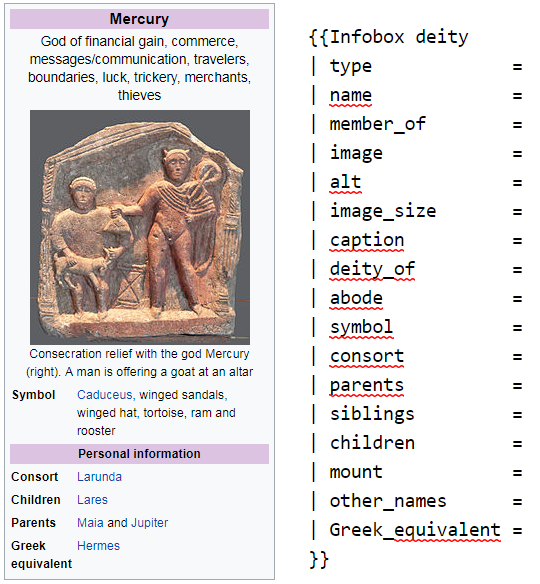
\includegraphics[width=0.8\linewidth]{mercury-infobox}
  \caption{Example Infobox of the page related to the god Mercury with the default properties for infoboxes about deities.}
  \label{fig:mercury-infobox}
\end{figure}



\subsubsection{\hspace*{3pt} Categories}

Every Wikipedia article should have at least one category. Categories are collections that identify topics in the encyclopedia. 

The category structure is not a tree. Therefore some categories have multiple supercategories, and one article can belong to several categories. In the same way as links, categories show a semantic structure between Wikipedia articles. 

It should be noted that although the structure of the Wikipedia category forms a taxonomy, it is not represented by a simple tree of categories and subcategories but, in fact, by a complex graph. This graph allows multiple categorizations of topics simultaneously, which means that one category may have multiple parents. The category "Semantics" is a good example of this complex structure since it is a subcategory of ``Grammar",  ``Linguistics", ``Concepts in logic", ``Semiotics", ``Philosophy of language" and others (see \ref{fig:semantics-category}).


\begin{figure}[H]
\centering
  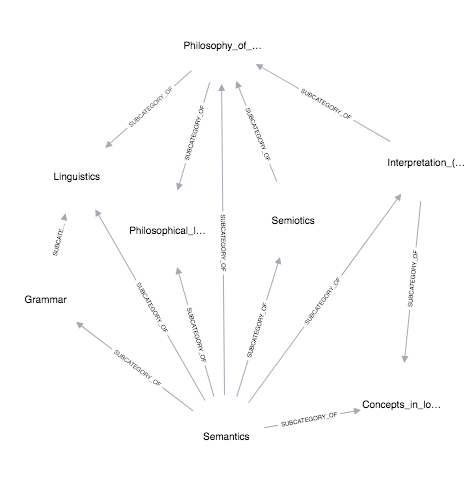
\includegraphics[width=0.8\linewidth]{graph-semantics}
  \caption{Example of an induced graph showing the supercategories of ``Semantics" in the Wikipedia Category Graph}
  \label{fig:semantics-category}
\end{figure}

Although not a semantic basis, Wikipedia has a set of characteristics, such as the definition of a large number of articles and organization of articles in categories, which makes an essential semantic resource.

A simple example, but one that illustrates well the complexity of the relationships between Wikipedia categories is the Apple concept (the fruit) , which is directly linked to four categories: ``Apples", ``Malus", ``Fruits originating in Asia," and ``Plants described in 1768". Each of these categories has been added and cured by people who are part of the Wikipedia community. In addition to the explicit knowledge in the directly attributed categories, a vast implicit knowledge can be inferred by the relations between them, both generically and in a specific way. If we take as starting point the category Apples, from the analysis of their links to the top of the classification, we perceive a more general case: Apples $\rightarrow$  Edible Fruits $\rightarrow$ Edible Plants $\rightarrow$ Food $\rightarrow$ Food and Drink $\rightarrow$ Health.
To illustrate a more specific case, let us take the Malus category as the origin and analyze one of the possible paths to the top: Malus $\rightarrow$ Maleae $\rightarrow$ Prunoideae $\rightarrow$ Rosaceae $\rightarrow$ Rosales $\rightarrow$ Rosids $\rightarrow$ Core Eudicots $\rightarrow$ Eudicots $\rightarrow$ Angiosperms $\rightarrow$ Plants $\rightarrow$ Eukaryota $\rightarrow$ Organisms $\rightarrow$ Life.
These are just examples of small fragments in Wikipedia's categorization structure for the Apple concept. The complete structure involves 33 different categories and 42 different relations between them (See figure \ref{fig:semantics-category-apple}).


\begin{figure}[H]
\centering
  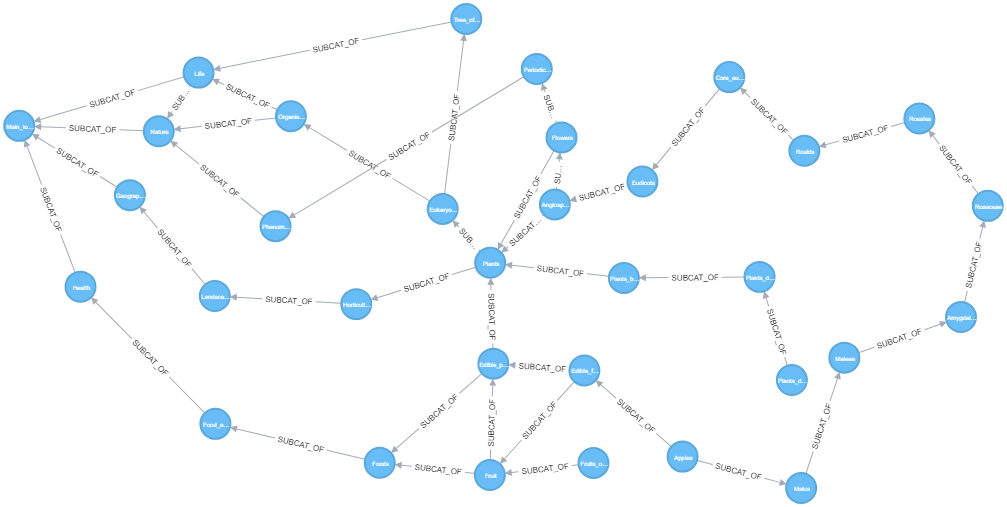
\includegraphics[width=0.8\linewidth]{graph}
  \caption{Example of an induced graph showing the categories and relationships for the Entity Apple towards Main topics}
  \label{fig:semantics-category-apple}
\end{figure}




%\subsection{\hspace*{3pt} Wikidata}

%Vrandecic \cite{vrandevcic2014wikidata} presents the Wikidata project as a free, collaborative, multilingual, structured data collection project to support Wikipedia and other initiatives. Wikidata differs from Wikipedia because in Wikipedia the content of articles is written in natural language, while the purpose of Wikidata is to collect structured data that can be reused by other systems, such as Wikipedia itself. 
%The central purpose of Wikidata in its conception was to serve as a knowledge base for the different editions of Wikipedia. The author cites an example of the demographic data present in articles about places: in Wikipedia, updating the population of a city must be done manually in the text of the article, for each language. With Wikidata, Wikipedia articles can reference the ``population" property of the city, and it is automatically synchronized. 

%All Wikidata items are identified by URIs using Semantic Web and Linked Data standards, returning the data in RDF and JSON formats. Douglas Adamsn, british writer, is identified by \gls{uri} \url{https://www.wikidata.org/entity/Q42}. Wikidata is connected to external datasets using URIs from repositories such as IMDb (Internet Movie Database) and Music-Brainz, as well as standards such as ISBN for book identification, ICD-9 for diseases, and ISO 639 for languages. The properties of an entity enable the addition of external sources that corroborate the verifiability of such information. In the Douglas Adams example, the property ``alma mater" has the value University of Cambridge, referencing as one of the sources of this information the page \url{http://www.nndb.com/people/731/000023662}. The different names by which an entity can be referenced are values of the ``Also known as" property, which can be used in Entity Disambiguation tasks. All Wikipedia articles in different languages that describe the same item are related to Wikidata, making it easier to obtain multilingual textual content.




\subsection{\hspace*{3pt} DBpedia}

As described directly on the DBpedia about page\footnote{url{https://wiki.dbpedia.org/about}} DBpedia is 

\begin{displayquote}
\say{
\textit{
a crowd-sourced community effort to extract structured content from the information created in various Wikimedia projects. This structured information resembles an open knowledge graph (OKG) which is available for everyone on the Web. A knowledge graph is a particular kind of database which stores knowledge in a machine-readable form and provides a means for information to be collected, organized, shared, searched and utilized.}
}
\end{displayquote}


The DBpedia dataset has many advantages compared to the raw data from Wikipedia. Besides the more convenient access to the underlying Wikipedia data sources, it also provides a higher data quality. The higher quality is because the extraction framework embeds multiple steps commonly found in data mining applications, such as duplicate removal in the form of mapping redundant infobox properties to the same DBpedia property.
Therefore, the present work is focussed on using DBpedia for the entity named recognition and Linking, as well as for traversing entities' categories.


\subsubsection{\hspace*{3pt} SPARQL}

\gls{sparql} is a query language capable of retrieving and manipulating data stored in the \gls{rdf} format that is the basis of the OWL language. \gls{rdf} is a labeled and directed data format used to represent information on the Web \cite{prud2008sparql}. 


%As a query language, \gls{sparql} is data-oriented, that is, there is no inference in the language itself. A SPARQL query consists of three parts \cite{arenas2011querying}:

%\begin{itemize}
%\item Pattern matching: includes several useful features for combining patterns, pattern matching, nesting, filtering, and the ability to choose the data source.

%\item Solution modifiers: allows modifying the values of the standard output by applying the classic operators, such as PROJECTION, LIMIT, DISTINCT, ORDER and OFFSET.

%\item Output: can be of different types, such as boolean, selections, graphs and resource descriptions.

%\end{itemize}

In the context of this research, our approach exploits a small part of what the SPARQL language can provide. We  navigate in the DBpedia hierarchy to retrieve broader semantic relations between the entities and its categories. 

%\subsubsection{Syntax}

%SPARQL has hundreds of elements that make up its syntax\cite{beckett1sparql}.  e will cover only the most essential elements in the context of this work. The purpose is to convey a fundamental notion about the construction and operation of SPARQL queries.
%A triple in RDF contains three components \cite {carroll2004resource}:

%\begin{itemize}


%\item Subject: can be individuals or ontology classes.
%\item Predicate: represent relationships and can be object properties, primitive properties, or some type of resource defined by the RDF version.
%\item Object: they are values of relations, they can be individuals, classes or primitive data.

%\end{itemize}

%A triple in \gls{rdf}  is conventionally written in the sequence: subject, predicate, object. The predicate is also known as triple property \cite{beckett1sparql}. The subject and the object are names for two ``things" in the world, and the predicate is the name of a relationship between the two.


%The syntax for triples \gls{sparql}  queries is based on triple \gls{rdf} , composed of a subject, a predicate, and an object:
%\\

%\begin{verbatim}
%PREFIX plants: <PLANT_ONTOLOGY_URI>
%SELECT * WHERE
%{
%?name plants:family "Rosaceae"
%}
%\end{verbatim}

%In the SPARQL query above <PLANT \_ONTOLOGY\_URI> \gls{uri}, the resource identifier of the ontology. PREFIX is the keyword that declares plants as an alias of the URI.  ?name is the subject, plants:family is the predicate and  ``Rosacea'' is the object. In this example, all the subjects present in the database whose class (predicate) of type \textit{family} has the value equals to ``Rosacea"




%\section{\hspace*{3pt}Evaluation of Classifiers}
%\label{sec:evaluation-of-classifiers}
%\subsection{\hspace*{3pt}Precision and Recall}
%\subsection{\hspace*{3pt}F-Measure}
%\subsection{\hspace*{3pt}Cross-Validation}
